\documentclass[a4paper, titlepage]{book} % type of document
\usepackage[T1]{fontenc}      % font encoding
\usepackage[utf8]{inputenc}   % sepcial chars from keyboard
\usepackage[english]{babel}   % document language

\usepackage{subfiles}
\usepackage{standalone}

\usepackage{graphicx}		  % images
\usepackage{wrapfig}          % wrapped figures
\usepackage{subfig}           % subfigures
\usepackage{caption}          % required by subfig 
\usepackage{subcaption}       % captions in subfigures

\usepackage{xcolor}           % colors
\usepackage{chemformula}      % chemical formulas
\usepackage{microtype}	      % font expansion and justification
\usepackage{comment}          % multi line comments
\usepackage{amsmath}          % math symbols
\usepackage{algorithm}        % algorithms
\usepackage{algpseudocodex}   % algorithm pseudocode
\usepackage[backend = biber, style=ieee]{biblatex}         % bibliograpy
\usepackage[]{csquotes} % quotations
\usepackage{siunitx}
\usepackage{physics}
%\usepackage{ulem}
%\usepackage{todonotes}

\usepackage[normal, onlyinclude]{frontespizio}

\makeatletter

\renewenvironment{displayquote}
{\begin{quote}\itshape}  % Begin with original quote environment and apply italics
{\end{quote}}  % End with original quote environment
%\usepackage{fancyhdr} %to make "better looking" page headers
%\pagestyle{fancy}

\usepackage{hyperref}
\hypersetup{hidelinks}

\graphicspath{ {./chapters/01_intro/imgs/} {./chapters/02_impl/imgs/} {./chapters/03_struct/imgs/} {./chapters/04_infer/imgs/} {./chapters/05_concl/imgs/} {./imgs}}
\newcommand{\julia}{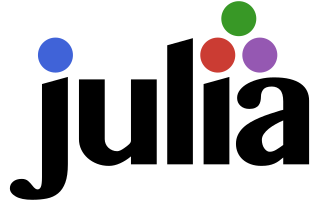
\includegraphics[height=0.7em]{julia-logo-color.png}}

\newcommand{\standalonebib}[1]{
        \IfFileExists{#1.bib}{
        % Standalone compilation
        \addbibresource{#1.bib}
    }{
        % Main document compilation
        \addbibresource{./chapters/#1/#1.bib}
    }
}


\addbibresource{./chapters/01_intro/01_intro.bib}
\addbibresource{./chapters/02_impl/02_impl.bib}
\addbibresource{./chapters/03_struct/03_struct.bib}
\addbibresource{./chapters/04_infer/04_infer.bib}
\addbibresource{./chapters/05_concl/05_concl.bib}


\title{
	{Collective Behaviors of Interacting Active Brownian Particles: Simulations and Analysis}\\
	{\large University of Pisa}\\
	%{\includegraphics{}}
}

\author{Niccolò Picchiarelli}
\date{\today}


\begin{document}
	
	\frontmatter
	%\maketitle
	
	\begin{frontespizio}

		\Universita{Pisa}
		\Dipartimento{Fisica}
		\Corso[Laurea Magistrale]{Fisica}
		\Titolo{Collective Behaviors of Interacting Active Brownian Particles: Simulations and Analysis}
		\Candidato{Niccolò Picchiarelli}
		\Relatore{Prof. Stefano Palagi}
		\Relatore{Prof. Riccardo Mannella}
		\Annoaccademico{2024-2025}
		\Logo{./imgs./logo_unipi.png}

	\end{frontespizio}
	
	\cleardoublepage
	\vspace*{\stretch{1}}
	\begin{flushright}
		{\itshape To Francesco and the man he will become}\\
	\end{flushright}
	\vspace{\stretch{2}}
	\newpage
	
		\section*{\textsc{acknowledgments}}
I thank my supervisor, Professor Stefano Palagi, for the support and guidance he gave me during my thesis work.
It has been my honor and pleasure to work in his group, to be led by him and to learn from him what it takes to be a scientist, a leader and ultimately, a remarkable human being.

I thank Dr. Jyoti Sharma for every piece of useful advice she has given me, not only for this thesis but also for my physics knowledge, my career, and my well-being.
She has been the most precise, helpful, and caring mentor during these months, and I will never forget it.
Experimental snapshots in chapter 2 are a courtesy of her as well.

I thank Professor Riccardo Mannella for the evaluation of the project and the extremely valuable advice and Professor Eleonora Russo for the useful conversations about machine learning.

I thank my fellow and colleague Rachele Porta, who was with me during this thesis, for the time and effort she dedicated to me when I was trying to explore the world of copper coated particles.
Also, she gave me the opportunity to share my thoughts and feelings throughout all the duration of my thesis and I hope to have given to her at least a fraction of the help she gave me.

All the people in Microscale Robotics Lab, my host lab, need to be thanked for their willingness to help and for their experience.
A page could be written about everyone of them since I learned something from each of them, but, most importantly, they thought me what it means to be a part of a loving and supporting group.
Here are their names, in alphabetical order by first name (Doctors will have to forgive me): Aliria Poliziani, Dario Cecchi, Elisa Roberti, Eugenia De Remigis, Fehmi Mustafa Dikbas, Federica Poli, Gaia Petrucci, Hilda Gomez Bernal, Michele Ibrahimi, Omar Tricinci, Yasmine Ferchichi, Yashpal Singh Brar.
Anna Chiara Bressi and my desk mate Alberto Lolli are not formally part of the group, but they deserve to be added to the list.

Mirko Binarelli takes the first non professional thank for his help in composing the figures in the last section of chapter 2 under the careful supervision of Giulia and, most importantly, for being the most kind and trustworthy friend.

My parents deserve so many words and they know better than me what I should write here.
So just thank you, Letizia and Daniele.
My aunt Silvia is my unreachable academic example, she deserves a thank here.
I promised not to write more than one page, so thank to all my family, with a special mention to Alessandro, my brother's father.

Chiara and Alessandro, or my Lab(rador) team, have been in this adventure with me from day one (of week two).
Thank you for sharing with me the dream of being physicists.
Gianluca, after some years I finally had the chance to return the great honor of being mentioned in your thesis.
Thank you, my brother, see you at the P\&P.
Giovanni, it's been twenty-two years now and I hope you'll be \emph{my-man} (\emph{miomo}) for the rest of my life.
Vittoria, during your graduation I learned what it means to feel at home in Pisa.
Gaetano, \emph{pres}, you already know.

Thank \emph{you}, I don't even know if you want to be here, you just deserve it for being part of this journey, and I am sorry, for I have been stupid enough to make you lose the finale.

Thanks to Società Astronomica Poliziana for giving me the chance to share my passion for science, thanks to Contrada Refenero, my identity, thanks to Gruppo Sbandieratori e Tamburini di Torrita di Siena, an adventure on its own.	
	
	\tableofcontents
	\listoffigures
	\listoftables
	
	\mainmatter
	\subfile{./chapters/01_intro/01_intro}

	\subfile{./chapters/02_impl/02_impl}
	
    \subfile{./chapters/03_struct/03_struct}
	
	\subfile{./chapters/04_infer/04_infer}
	
	\subfile{./chapters/05_concl/05_concl}
	
	\backmatter
	\printbibliography
\end{document}